\begin{align}
\vec{V}=\myvec{a&b\\b&c}=\myvec{-2&\frac{1}{2}\\\frac{1}{2}&1}\\
\vec{u}=\myvec{d\\e}=\myvec{\frac{-5}{2}\\\frac{-1}{2}}\\
f=-2
\end{align}
\begin{align}
\mydet{
-2&\frac{1}{2}&\frac{-5}{2}\\
\frac{1}{2}&1&\frac{-1}{2}\\
\frac{-5}{2}&\frac{-1}{2}&-2}
\xleftrightarrow[R_1\rightarrow R_1+R_3]{R_1\rightarrow R_1-R_2}
\mydet{
0&0&0\\
\frac{1}{2}&1&\frac{-1}{2}\\
\frac{-5}{2}&\frac{-1}{2}&-2}=0
\end{align}
Hence it represents the pair of straight lines.
Now two intersecting lines are obtained when
\begin{align}
\mydet{V} < 0 
\implies \mydet{-2&\frac{1}{2}\\\frac{1}{2}&1}
=\frac{-9}{4} < 0
\end{align}
Let the pair of straight of lines be given by
\begin{align}
\vec{n_1}^T\vec{x}=c_1\\
\vec{n_2}^T\vec{x}=c_2
\end{align}
The slopes of the lines are given by the roots of the polynomial 
\begin{align}
cm^2+2bm+a=0 \\
m_1,m_2 = \frac{-\frac{1}{2}\pm\sqrt{\frac{9}{4}}}{1}\\
m_1= 1 , m_2 =-2\\
\implies\vec{n_1}=\myvec{-1\\1} and \vec{n_2}=\myvec{2\\1}
\end{align}
\begin{align}
(\vec{n_1}^T\vec{x}-c_1)(\vec{n_2}^T\vec{x}-c_2) =
\vec{x}^T\vec{V}\vec{x}+2\vec{u}^T\vec{x}+f 
\end{align}
\begin{align}
c_2\vec{n_1}+c_1\vec{n_2} =-2\vec{u}
 \end{align}
 \begin{align}
 c_2\myvec{-1\\1}+c_1\myvec{2\\1} =-2\myvec{\frac{-5}{2}\frac{-1}{2}}
 \end{align}
 \begin{align}
 \myvec{1&1\\2&-1}\myvec{c_1\\c_2}=\myvec{1\\5}
 \end{align}
 Using row reduction we get
 \begin{align}
\myvec{1&1&1\\2&-1&5}\\
\xleftrightarrow[R_2\leftarrow R_2/-3]{R_2\leftarrow R_2-2R_1}
\myvec{1&1&1\\0&1&-1}\\\xleftrightarrow[]{R_1\leftarrow R_1-R_2}
\myvec{1&0&2\\0&1&-1}
\end{align}
\begin{align}
C  =\myvec{2\\-1}
\end{align}
 The convolution of the normal vectors, should satisfy the below condition
 \begin{align}
    \myvec{-1\\1}*\myvec{2\\1}=\myvec{a\\2b\\c}
\end{align}
The LHS part of equation(2.0.20) can be rewritten using toeplitz matrix as
\begin{align}
    \myvec{-1&0\\1&-1\\0&1}\myvec{2\\1}=\myvec{-2\\1\\1}=\myvec{a\\2b\\c}
\end{align}
Therefore the equation of lines is given by 
\begin{align}
\myvec{-1&1}\vec{x}=2\\
\myvec{2&1}\vec{x}=-1
\end{align}
consider the augmented matrix
\begin{align}
\myvec{-1&1&2\\2&1&-1}\\
\xleftrightarrow[R_2\leftarrow R_2-2R_1]{R_1\leftarrow -R_1}
\myvec{1&2&1\\0&1&1}\\\xleftrightarrow[R_1\leftarrow R_1+R_2]{R_1\leftarrow R_1/3}
\myvec{1&0&-1\\0&1&1}
\end{align}
Therefore point of intersection is $\vec{A}=\myvec{-1\\1}.$
\\
Angle between two lines $\theta$ can be given by
\begin{align}
\cos\theta =\frac{\vec{n_1}^T\vec{n_2}}{\norm{\vec{n_1}}\norm{\vec{n_2}}}\\
 \cos\theta=\frac{\myvec{-1&1}\myvec{2\\1}}{\sqrt{\left(1\right)^2 +1} \times \sqrt{(2)^2 +1}}
\end{align}
\begin{align}
\theta = \cos^{-1}(\frac{-1}{\sqrt{10}})\implies \theta = tan^{-1}3
\end{align}
\begin{figure}[!ht]
\centering
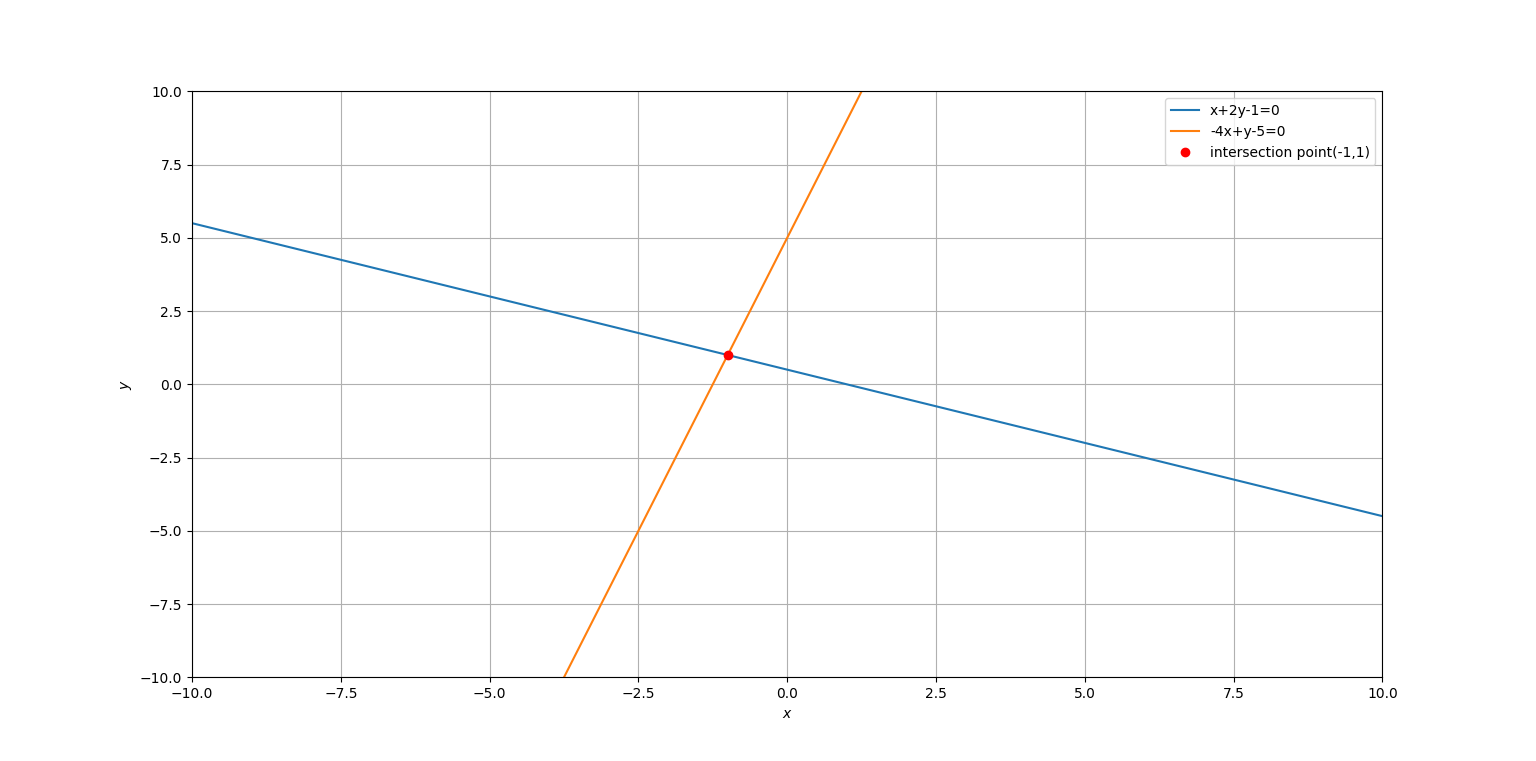
\includegraphics[width=\columnwidth]{./solutions/13/4/Figure_2.png}
\caption{plot showing intersection of lines}
\label{Fig:solutions/13/4}
\end{figure}
